% Dmitry Mikushin, USI Lugano, dmitry.mikushin@usi.ch,
% using portions of original style file by Tom Cashman
%
% IMPORTANT NOTICE:
%
% The USI logo is unique; it is authorized for use only by employees of the
% Università della Svizzera italiana for work-related projects; others can use them
% ONLY with prior authorization (contact: press@usi.ch).
%
% http://www.press.usi.ch/en/corporate-design/corporate-design-stampa.htm
%
% This is an example beamer presentation, which uses Università della Svizzera italiana
% design theme.

\documentclass{beamer}

\usetheme{usi}

\usepackage{comment}
\usepackage{tikz}
\usepackage{listingsutf8}
\usepackage{xcolor}
\usepackage{beramono}
\usepackage{polyglossia}

\defaultfontfeatures{Scale=MatchLowercase, Mapping=tex-text}

\usetikzlibrary{shapes,arrows}
\usetikzlibrary{shadows}

\setmainfont{Trebuchet MS}
\setsansfont{Trebuchet MS}
\setmonofont{Ubuntu}

\lstset{
    inputencoding=utf8,
%    backgroundcolor=\color{white},
    tabsize=4,
    rulecolor=,
    upquote=true,
%    aboveskip={1.5\baselineskip},
    columns=fixed,
    showstringspaces=false,
    extendedchars=true,
    breaklines=true,
    prebreak = \raisebox{0ex}[0ex][0ex]{\ensuremath{\hookleftarrow}},
    frame=single,
    showtabs=false,
    showspaces=false,
    showstringspaces=false,
    basicstyle=\scriptsize\ttfamily,
    identifierstyle=\ttfamily,
    keywordstyle=\ttfamily\color[rgb]{0,0,1},
    commentstyle=\ttfamily\color[rgb]{0.133,0.545,0.133},
    stringstyle=\ttfamily\color[rgb]{0.627,0.126,0.941},
}

\makeatletter
\newenvironment{btHighlight}[1][]
{\begingroup\tikzset{bt@Highlight@par/.style={#1}}\begin{lrbox}{\@tempboxa}}
{\end{lrbox}\bt@HL@box[bt@Highlight@par]{\@tempboxa}\endgroup}

\newcommand\btHL[1][]{%
  \begin{btHighlight}[#1]\bgroup\aftergroup\bt@HL@endenv%
}
\def\bt@HL@endenv{%
  \end{btHighlight}%   
  \egroup
}
\newcommand{\bt@HL@box}[2][]{%
  \tikz[#1]{%
    \pgfpathrectangle{\pgfpoint{1pt}{0pt}}{\pgfpoint{\wd #2}{\ht #2}}%
    \pgfusepath{use as bounding box}%
    \node[anchor=base west, fill=usi@yellow,outer sep=0pt,inner xsep=1pt, inner ysep=0pt, rounded corners=3pt, minimum height=\ht\strutbox+1pt,#1]{\raisebox{1pt}{\strut}\strut\usebox{#2}};
  }%
}
\makeatother

\lstdefinestyle{markable}{
    moredelim=**[is][\btHL]{`}{`},
}

\title[STENFW]{STENFW -- a stencil framework for compilers benchmarking}
%\subtitle{And even a subtitle!}
%\author{Dmitry Mikushin}
\institute{\href{mailto:dmitry.mikushin@usi.ch}{dmitry.mikushin@usi.ch}}
\date{\today}

\begin{document}
\begin{frame}
\titlepage
\end{frame}

\begin{frame}{Description}

STENFW is intended to ease the evaluation of different compiler suites like DSLs, automatic parallel code generators or conventional compilers. The framework is structured to keep the stencils implementations separated from the rest of the test suite, which handles MPI/CUDA management and visualization.

\vskip 15pt

This is preview version. Comments on improving the code structure are highly appreciated!

\end{frame}

\begin{frame}[fragile]{Code structure}
\begin{itemize}
\item \textbf{data2vdf} -- data converter for visualizer
\item \textbf{doc} -- some documentation
\item \textbf{generators} -- inital data generators
\item \textbf{grid} -- the grid decomposition engine
\item \textbf{stencils} -- the stencils implementations, each stencil in its own subfolder
\item \textbf{tests} -- test applications, that use stencils
\item \textbf{timing} -- time measurement routines
\end{itemize}
\end{frame}

\begin{frame}[fragile]{Building}
\begin{lstlisting}
$ tar -xf stenfw_120620153943.tar.gz 
$ cd stenfw
$ mkdir build
$ cd build/
$ cmake -DCMAKE_BUILD_TYPE="Release" ..
$ make
\end{lstlisting}
%$
\end{frame}

\begin{frame}[fragile]{Build options}
\begin{itemize}
\item[] СMake build script supports the following mode switches:
\begin{itemize}
\item \textbf{HAVE\_MPI} -- enable or disable MPI support 
\item \textbf{HAVE\_CUDA} -- enable or disable CUDA support, performing explicit host-device data transfers by default, or add:
\begin{itemize}
\item \textbf{HAVE\_CUDA\_MAPPED} -- to use \emph{host-mapped} memory directly accessible from the GPU kernels
\item \textbf{HAVE\_CUDA\_PINNED} -- to perform explicit host-device data transfers in \emph{pinned} memory
\end{itemize}
\item \textbf{HAVE\_VISUALIZE} -- turn on the debug visualization based on UCAR Vapor, external runtime libraries needed
\end{itemize}
\item[] Example:
\begin{lstlisting}
$ cmake -DHAVE_MPI=ON -DHAVE_CUDA=ON -DHAVE_CUDA_MAPPED=ON -DHAVE_VISUALIZE=ON -DCMAKE_BUILD_TYPE="Release" ..
$ make
\end{lstlisting}
\item[] Note the combination of \textbf{HAVE\_MPI} and \textbf{HAVE\_CUDA} currently can work only together with \textbf{HAVE\_CUDA\_MAPPED}
\end{itemize}
\end{frame}

\begin{frame}[fragile]{Test command line}
The command line options change, depending on enabled features:
\begin{itemize}
\item Without MPI and GPU:
\begin{lstlisting}
$ ./wave13pt
Usage: ./wave13pt <n> <nt>
where <n> and <nt> must be positive
\end{lstlisting}
%$
\item Without MPI, with GPU:
\begin{lstlisting}
$ ./wave13pt
Usage: ./wave13pt <n> <nt> <CPU|GPU>
where <n> and <nt> must be positive
\end{lstlisting}
%$
\end{itemize}
\end{frame}

\begin{frame}[fragile]{Test command line}
The command line options change, depending on enabled features:
\begin{itemize}
\item With MPI, without GPU:
\begin{lstlisting}
$ ./wave13pt
Usage: ./wave13pt <n> <nt> <sx> <sy> <ss>
where <n> and <nt> must be positive
and <sx> * <sy> * <ss> must equal to the number of MPI processes
\end{lstlisting}
%$
\item With MPI and GPU:
\begin{lstlisting}
$ ./wave13pt
Usage: ./wave13pt <n> <nt> <sx> <sy> <ss> <CPU|GPU>
where <n> and <nt> must be positive
and <sx> * <sy> * <ss> must equal to the number of MPI processes
\end{lstlisting}
%$
\end{itemize}
\end{frame}

\begin{frame}[fragile]{Testing example}
Test \emph{wave13pt} stencil on 2 GPUs used by 2 MPI processes:
\begin{lstlisting}
$ cd bin/
$ mpirun -np 2 ./wave13pt 64 64 2 1 1 GPU
Mapping problem grid 64 x 64 x 64 onto 2 x 1 x 1 compute grid
step 0
...
min and max values of data output: -0.421547, 0.421548
\end{lstlisting}
\end{frame}
%$

\begin{frame}[fragile]{Visualizing with UCAR Vapor}
\begin{enumerate}
\item Login with \textbf{\$ ssh -X} to enable graphics forwarding
\item Execute /export/opt/vapor/vaporgui
\item Load the build/<stencil>.vdf dataset into the current session of UCAR Vapor.
\end{enumerate}
\begin{center}
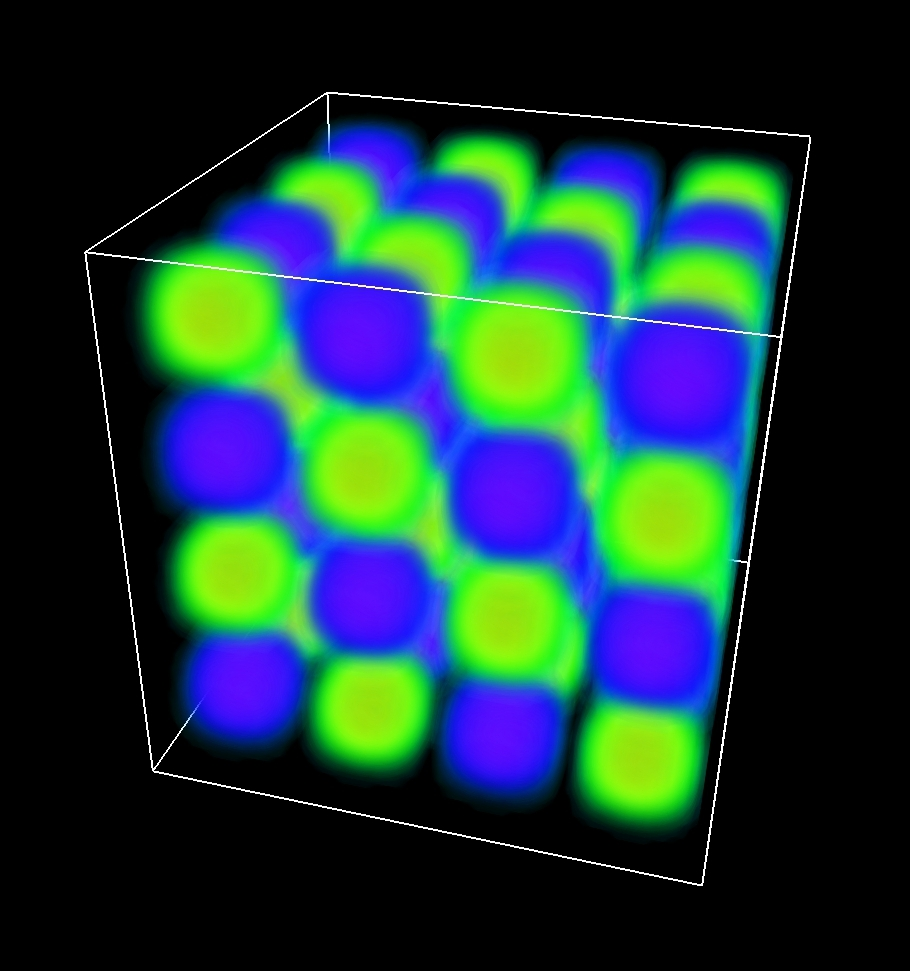
\includegraphics[width=3.8cm]{wave13pt}
\end{center}
\end{frame}

\begin{frame}[fragile]{Visualizing with UCAR Vapor}
\begin{enumerate}
\setcounter{enumi}{3}
\item Select ``3DTexture'' for render type
\item Check ``Instance1'' box
\item Delete the default linear opacity widget and replace it with inverted Gaussian
\end{enumerate}
\begin{center}
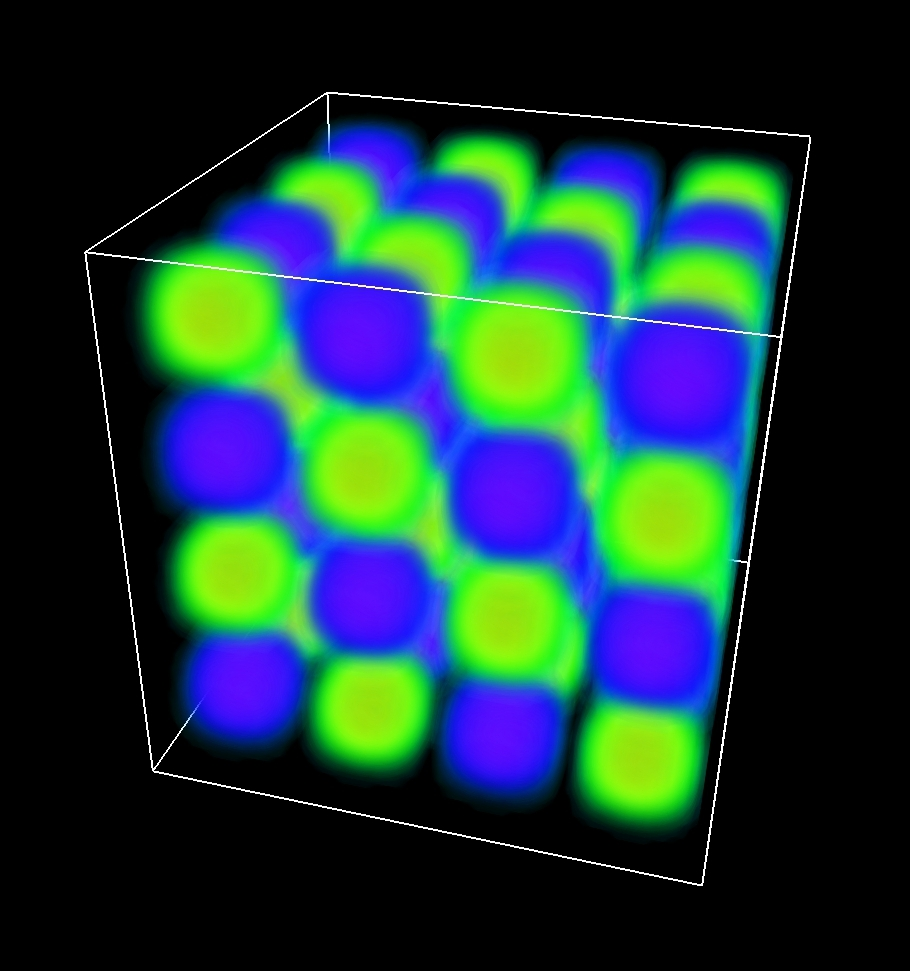
\includegraphics[width=3.8cm]{wave13pt}
\end{center}
\end{frame}

\begin{frame}[fragile]{Batch testing}
STENFW comes with a tiny batch testing Perl script to ensure new changes do not break all supported configurations:
\begin{lstlisting}
$ ./test
\end{lstlisting}
%$
\end{frame}

\begin{frame}[fragile]{Debugging for correctness}
\begin{itemize}
\item STENFW has a special stencil \emph{isum13pt}, which tests the exact correctness of the parallel version result against serial version result on integer data
\item Useful for debugging MPI or CUDA bugs
\item Has embedded 2d visualization system to present the results difference (images will be placed into bin/ folder)
\end{itemize}
\begin{lstlisting}
$ mpirun -np 2 ./isum13pt 64 64 1 1 2 CPU
Mapping problem grid 64 x 64 x 64 onto 1 x 1 x 2 compute grid
step 2 time = 0.005935042 sec
0.000000% different, max = 0 @ 262143
step 3 time = 0.005831204 sec
5.493164% different, max = 42 @ 134674
step 4 time = 0.005971761 sec
...
\end{lstlisting}
%$
\end{frame}

\begin{frame}[fragile]{Testing on GraphIT!}
\begin{lstlisting}
$ tar -xf stenfw_120704165836.tar.gz 
$ cd stenfw
$ mkdir build
$ cd build/
$ cmake -DHAVE_MPI=ON -DHAVE_CUDA=ON -DHAVE_CUDA_MAPPED=ON -DHAVE_VISUALIZE=ON -DCMAKE_BUILD_TYPE="Release" ..
$ OMPI_CC=gcc OMPI_CXX=g++ make
$ cleo-submit -np 2 ./test_wave13pt 64 64 2 1 1 CPU
$ cleo-submit -np 2 ./test_wave13pt 128 128 2 1 1 GPU
\end{lstlisting}
\end{frame}

\begin{frame}[fragile]{Exercise}
\begin{itemize}
\item[] Currently kernel in \textbf{wave13pt\_gpu.cu} in invoked on a very simple compute grid, without blocks:
\begin{lstlisting}[language=c]
extern "C" int wave13pt_gpu(int nx, int ny, int ns,
	const real c0, const real c1, const real c2,
	real* w0, real* w1, real* w2)
{
	wave13pt_gpu_kernel<<<dim3(nx - 4, ny - 4, 1), ns - 4>>>(nx, ny, ns, c0, c1, c2, w0, w1, w2);
	CUDA_SAFE_CALL(cudaDeviceSynchronize());
	return 0;
}
\end{lstlisting}
\item[] \textbf{Task for entering certification process:} Reimplement kernel code and kernel invocation in a way that it could utilize compute grid blocks of \emph{arbitary} size (parameter or preprocessor symbol BLOCK\_SIZE), and the program in the same time could correctly handle \emph{arbitary} problem dimensions. Example:
\begin{lstlisting}
; BLOCK_SIZE=32
$ ./test_wave13pt 113 64 4 1 1 GPU
\end{lstlisting}
\end{itemize}
\end{frame}

\end{document}
